\section{Stiner Tree}
\subsection{SPT}
Our SPT tree is:
\begin{center}
    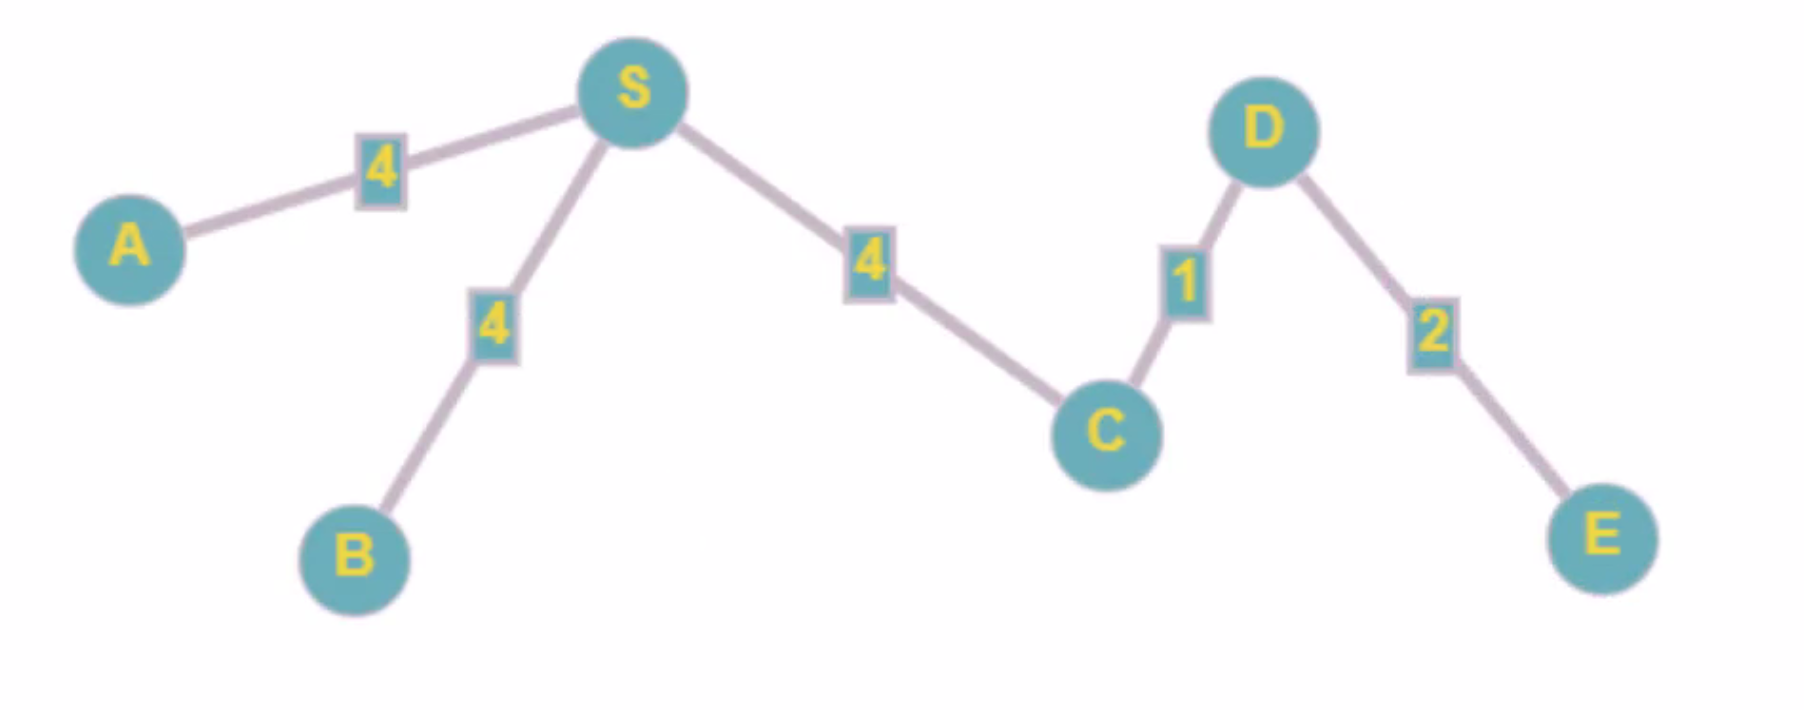
\includegraphics[width=0.6 \textwidth]{resources/q3-1.png}\centering
\end{center}
And it's weight is 15.\\
The maximal weight of a path from the source is that of the path to E,
which is 7.

\subsection{Huristic Algorithm}
The resulting clique is:
\begin{center}
    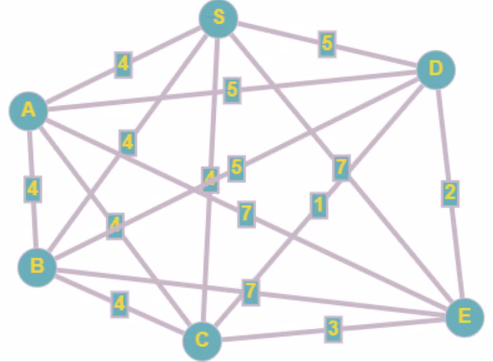
\includegraphics[width=0.6 \textwidth]{resources/q3-3.png}\centering
\end{center}
And a minimum spanning tree we have found for it is:
\begin{center}
    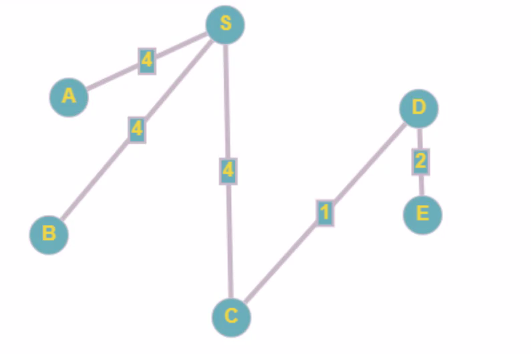
\includegraphics[width=0.6 \textwidth]{resources/q3-4.png}\centering
\end{center}
Where the weight of the maximum path is 7. 

\begin{figure}
    \begin{center}
        
\includegraphics[width=0.6 \textwidth]{resources/q3-2.png}\centering
    \end{center}
    \caption{Algorithms...}
\end{figure}


\subsection{Stiener Tree}
The Stiener Tree is:
\begin{center}
    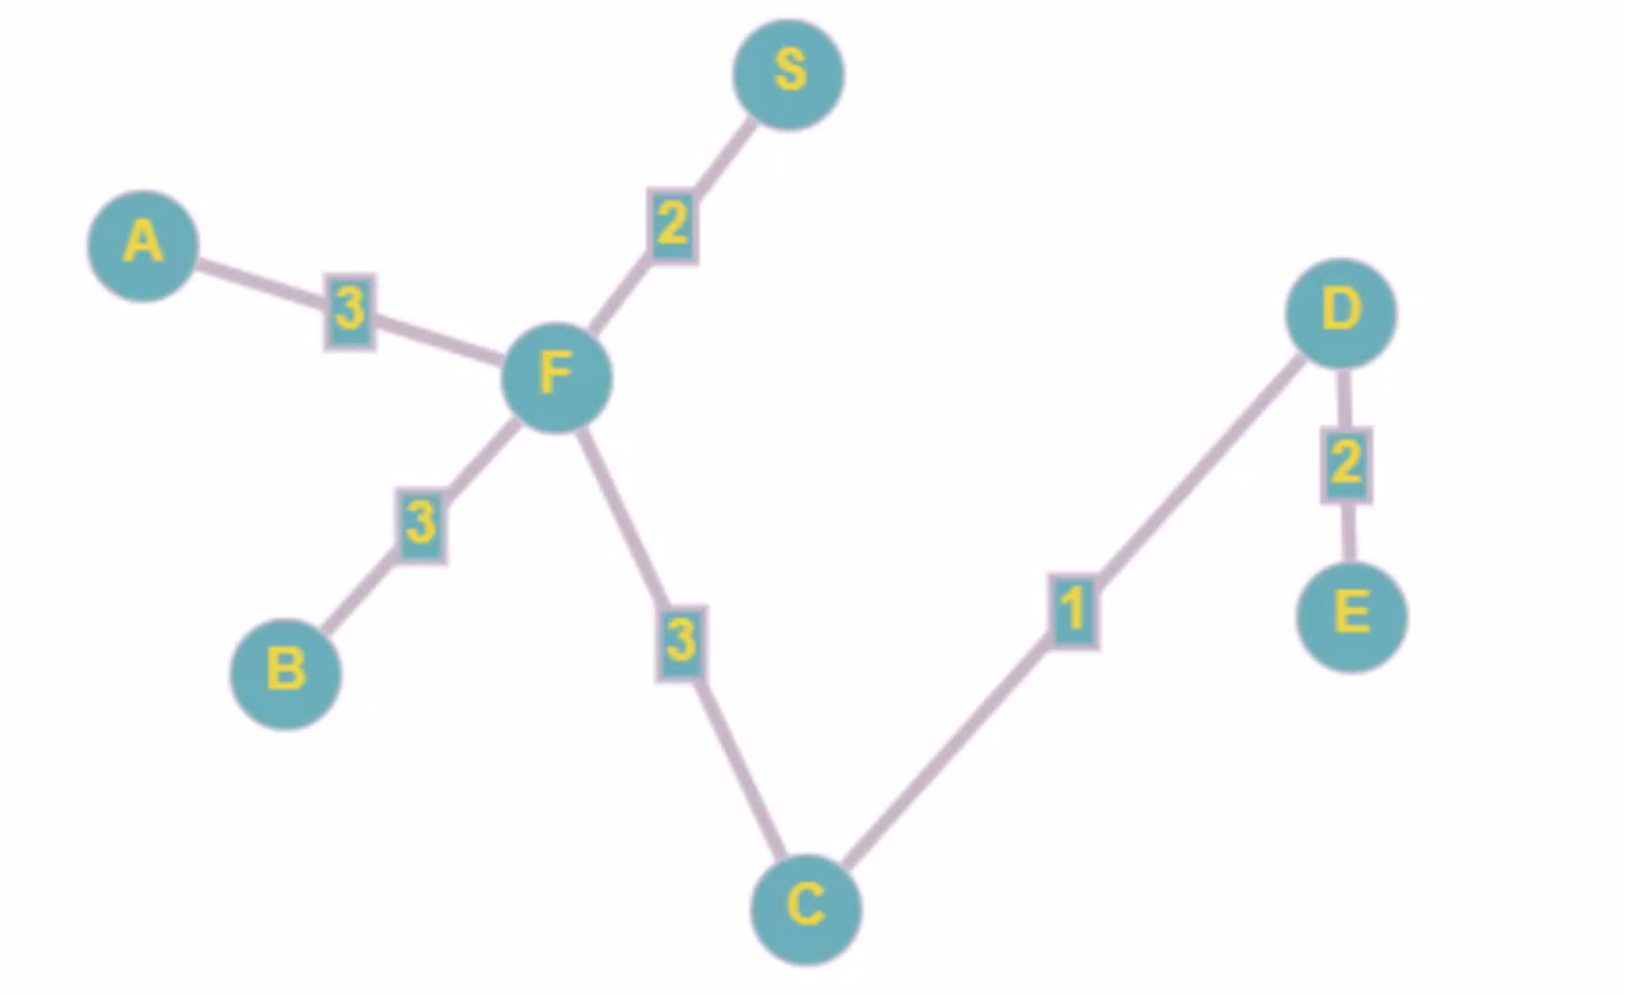
\includegraphics[width=0.6 \textwidth]{resources/q3-5.png}\centering
\end{center}
It's weight is 14, the maximal path weight is 8 
- that path is $S\rightarrow F\rightarrow C\rightarrow D\rightarrow E$.

\subsection{Stiner Vs Huristic}
The Huristic trees are (much) easier to find
\footnote{finding a stiner tree is an NP-Complete problem},
and in some cases the might also have
have a shorter longest path between two nodes (such as we can see in the prior example),
and the advantage of the Stiner trees is that they guarantee (by definition)
that they have the lower total weight.